\chude{LẬP PHƯƠNG TRÌNH TỔNG QUÁT MẶT PHẲNG}
Để lập phương trình tổng quát của mặt phẳng $\left(\alpha\right)$ thông thường ta có 3 trường hợp cơ bản sau:\\
$\textbf{Trường hợp 1:}$ Khi bài toán cho biết mặt phẳng $\left(\alpha\right)$ đi qua điểm $M_0 \left(x_0;y_0;z_0\right)$ và có một véc-tơ pháp tuyến $\overrightarrow{n} = \left(A;B;C\right)$ hoặc có hai véc-tơ chỉ phương $\overrightarrow{a}$, $\overrightarrow{b}$ (với $\overrightarrow{n} = \left[\overrightarrow{a},\overrightarrow{b}\right]$) thì viết dưới dạng sau:
$$\left(\alpha\right) \colon A\left(x-x_0\right)+B\left(y-y_0\right)+C\left(z-z_0\right)=0$$
$\textbf{Trường hợp 2:}$ Khi bài toán cho biết mặt phẳng $\left(\alpha\right)$ có một véc-tơ pháp tuyến $\overrightarrow{n} = \left(A;B;C\right)$ hoặc có hai véc-tơ chỉ phương $\overrightarrow{a}$, $\overrightarrow{b}$ (với $\overrightarrow{n} = \left[\overrightarrow{a},\overrightarrow{b}\right]$) và không tìm được điểm $M_0 \left(x_0;y_0;z_0\right) \in \left(\alpha\right)$ thì ta thực hiện các bước sau:
\begin{itemize}
\item $\textbf{Bước 1:}$ Viết phương trình mặt phẳng $\left(\alpha\right)$ dưới dạng:
$$Ax+By+Cz+D=0$$
\item $\textbf{Bước 2:}$ Sau đó dựa vào giả thiết bài toán để tìm giá trị $D$.
\end{itemize}
\begin{note}
Dạng này, giả thiết có liên quan đến khoảng cách và góc liên quan đến mặt phẳng.
\end{note}
$\textbf{Trường hợp 3:}$ Khi bài toán cho biết mặt phẳng $\left(\alpha\right)$ đi qua điểm $M_0 \left(x_0;y_0;z_0\right)$ và giả thiết bài toán không cho véc-tơ pháp tuyến $\overrightarrow{n}$ hoặc không cho hai véc-tơ chỉ phương $\overrightarrow{a}$, $\overrightarrow{b}$ thì ta thực hiện các bước sau:
\begin{itemize}
\item $\textbf{Bước 1:}$ Gọi véc-tơ pháp tuyến của mặt phẳng $\left(\alpha\right)$ là $\overrightarrow{n} = \left(A;B;C\right)$ với $A^2+B^2+C^2 \neq 0$
\item $\textbf{Bước 2:}$ Viết phương trình mặt phẳng $\left(\alpha\right)$ dưới dạng:
$$\left(\alpha\right) \colon A\left(x-x_0\right)+B\left(y-y_0\right)+C\left(z-z_0\right)=0$$
\item $\textbf{Bước 3:}$ Sau đó dựa vào giả thiết bài toán để tìm hai phương trình chứa $3$ ẩn $A$, $B$, $C$.
\begin{note}
\begin{itemize}
\item Dạng này, giả thiết có liên quan đến khoảng cách và góc liên quan đến mặt phẳng
\item Để giải tìm véc-tơ pháp tuyến của mặt phẳng đơn giản hơn thì gọi véc-tơ pháp tuyến của mặt phẳng là $\overrightarrow{n} = \left(1;B;C\right)$.
\end{itemize}
\end{note}
\end{itemize}

\begin{dang}{VIẾT PHƯƠNG TRÌNH TỔNG QUÁT MẶT PHẲNG KHI BIẾT MỘT ĐIỂM THUỘC MẶT PHẲNG VÀ MỘT VÉC-TƠ PHÁP TUYẾN HOẶC HAI VÉC-TƠ CHỈ PHƯƠNG}
1. Lập phương trình tổng quát của mặt phẳng đi qua điểm $M_0 \left(x_0;y_0;z_0\right)$ và biết một véc-tơ pháp tuyến $\overrightarrow{n} = \left(A;B;C\right)$\\
Trong KG $Oxyz$, phương trình tổng quát của mặt phẳng đi qua điểm $M_0 \left(x_0;y_0;z_0\right)$ và có véc-tơ pháp tuyến $\overrightarrow{n}= \left(A;B;C\right)$ là:\\
$$A\left(x-x_0\right) + B\left(y-y_0\right)+C\left(z-z_0\right) = 0$$
hay $Ax+By+Cz+D=0$ với $D= -Ax_0-By_0-Cz_0$
\begin{center}
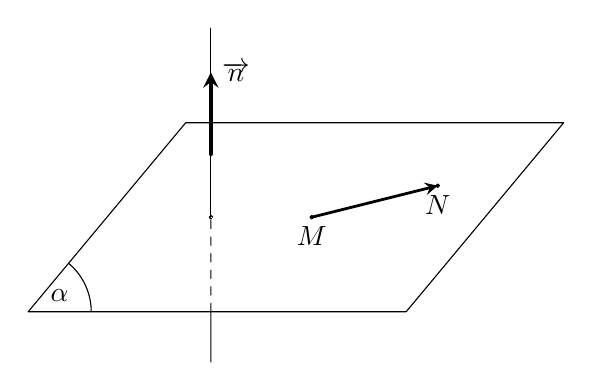
\begin{tikzpicture}[>=stealth,line join=round, line cap=round, scale=0.8]
        \coordinate (A) at (1.5,3);
		\coordinate (B) at (-1,0);
		\coordinate (C) at (5,0);
		\coordinate (D) at (7.5,3);
  \coordinate (I) at (1.9,1.5); \coordinate (J) at (1.9,4.5); \coordinate (K) at (1.9,-0.8);
  \coordinate (M) at (3.5,1.5);
  \coordinate (N) at (5.5,2);
\begin{scope}
\clip (A)--(B)--(C);
\draw (B) circle (1);
\end{scope}
   \draw (A)--(B)--(C)--(D)--(A);
   \draw (-0.8,0) node[above right]{$\alpha$};
   \draw (K)--(1.9,0); \draw [dashed] (1.9,0)--(I) circle (.8pt);  \draw (I)--(J);
   \draw (M) node[below]{$M$} circle (.8pt)--(N) node[below]{$N$} circle (.8pt);
   \draw[->,line width=1] (M)--(N);
    \draw[->,line width=1.4] (1.9,2.5)--(1.9,3.8) node[right]{$\overrightarrow{n}$};
\end{tikzpicture}
\end{center}
$\textbf{Chú ý:}$
\begin{enumerate}[a.]
\item Phải nắm vững khái niệm $\textbf{véc-tơ pháp tuyến}$ và $\textbf{véc-tơ chỉ phương}$ của mặt phẳng.
\begin{itemize}
\item Véc-tơ pháp tuyến của mặt phẳng là vec-tơ có giá vuông góc với mặt phẳng đó. Nếu $\overrightarrow{n}$ là một véc-tơ pháp tuyến của mặt phẳng thì $k\overrightarrow{n}$ ($k \neq 0)$ cũng là một vectơ pháp tuyến của mặt phẳng đó.
\item Vec-tơ chỉ phương của mặt phẳng là vec-tơ có giá song song với mặt phẳng đó. Nếu $\overrightarrow{a}$ là một véc-tơ chỉ phương của mặt phẳng thì $k\overrightarrow{a}$ cũng là một véc-tơ chỉ phương của mặt phẳng đó.
\end{itemize}
\item Mặt phẳng $\left(\alpha\right)$ có cặp véc-tơ chỉ phương $\overrightarrow{a}$, $\overrightarrow{b}$ ($\overrightarrow{a}$, $\overrightarrow{b}$ không cùng phương) thì mặt phẳng $\left(\alpha\right)$ có véc-tơ pháp tuyến $\overrightarrow{n}= \left[\overrightarrow{a},\overrightarrow{b}\right]$.
\item Mặt phẳng $\left(\alpha\right)$ đi qua ba điểm $A$, $B$, $C$ không thẳng hàng thì có cặp véc-tơ chỉ phương $\overrightarrow{AB}$, $\overrightarrow{AC}$ nên mặt phẳng $\left(\alpha\right)$ có véc-tơ pháp tuyến $\overrightarrow{n} = \left[\overrightarrow{AB}, \overrightarrow{AC}\right]$.
\item Dựa vào tính chất vuông góc, song song giữa mặt phẳng với mặt phẳng, giữa đường thẳng với mặt phẳng trong không gian để tìm véc-tơ chỉ phương, véc-tơ pháp tuyến của mặt phẳng cần lập.
\begin{itemize}
\item Hai mặt phẳng song song thì có cùng véc-tơ pháp tuyến.
\item Hai mặt phẳng vuông góc thì véc-tơ chỉ phương của mặt phẳng này là véc-tơ pháp tuyến của mặt phẳng kia.
\item Đường thẳng song song mặt phẳng thì véc-tơ chỉ phương của đường thẳng là véc-tơ chỉ phương của mặt phẳng.
\item Đường thẳng vuông góc mặt phẳng thì véc-tơ chỉ phương của đường thẳng là véc-tơpháp tuyến của mặt phẳng.
\end{itemize}
\end{enumerate}
2. Các trường hợp đặc biệt của mặt phẳng
\begin{enumerate}[a.]
\item Phương trình mặt phẳng theo đoạn chắn\\
Mặt phẳng $\left(\alpha\right)$ không đi qua gốc tọa độ $O$ và lần lượt cắt trục $Ox$ tại $A \left(a;0;0\right)$, cắt trục $Oy$ tại $B \left(0;b;0\right)$, cắt trục $Oz$ tại $C \left(0;0;c\right)$ có $\textbf{phương trình mặt phẳng theo đoạn chắn}$ là: $\dfrac{x}{a}+\dfrac{y}{b}+\dfrac{z}{c}=1$ với $a \cdot b \cdot c \neq 0$
\begin{center}
\begin{tikzpicture}[>=stealth,line join=round, line cap=round, scale=0.7]
    \coordinate (O) at (0,0); 
    \coordinate (A) at (-1.9,-1.9); \coordinate (C) at (0,3); \coordinate (B) at (3,0);
        \path[name path=trucy] (O)--(5,0);
        \path[name path=d1] (A)--(C);
        \path[name path=d2] (B)--(C);
        \path[name path=d3] (A)--(B);
		\path[name path=trucz] (O)--(0,5); \path[name path=trucx] (O)--(-4,-4);
 \path[name intersections={of=d1 and trucz, by=I}];  
  \path[name intersections={of=d1 and trucx, by=J}];
  \path[name intersections={of=d2 and trucy, by=K}]; 
  \draw [fill = blue!5] (I)--(J)--(K)--(I);
  \draw [->] (I)--(0,5) node[right]{$z$};\draw [->] (K)--(4,0) node[above right]{$y$}; \draw [->] (J)--(-3,-3) node[right]{$x$};
   \draw [dashed] (O) node[below]{$O$} circle (.8pt)--(I) node[left]{$C(0;0;c)$};
  \draw [dashed] (O)--(J) node[above left]{$A(a;0;0)$};
  \draw [dashed] (O)--(K) node[below right]{$B(0;b;0)$};
\end{tikzpicture} 
\end{center}
\item Phương trình mặt phẳng đặc biệt\\
Xét phương trình mặt phẳng $\left(\alpha\right) \colon Ax+By+Cz+D=0$ với $A^2+B^2+C^2 \neq 0$
\begin{itemize}
\item Nếu $D = 0$ thì mặt phẳng $\left(\alpha\right)$ đi qua gốc tọa độ $O$ và có dạng $\left(\alpha\right) \colon Ax+By+Cz=0$.
\begin{center}
\begin{tikzpicture}[>=stealth,line join=round, line cap=round, scale=0.8]
%p1
\coordinate (O) at (0,0); 
\coordinate (x) at (-2,-2); 
\coordinate (y) at (4,0); 
\coordinate (z) at (0,3.5); 
%p2
\draw [->] (O) node[below]{$O$}--(x) node[below right]{$x$}; 
\draw [->] (O)--(y) node[below]{$y$}; 
\coordinate (A) at (3.3,2.5); \coordinate (B) at (-3,2);
\draw [fill = blue!5] (A)--(O)--(B)--cycle;
 \path[name path=d1] (A)--(B);
 \path[name path=d2] (O)--(z);
 \path[name intersections={of=d1 and d2, by=M}];
 \draw [->] (M)--(z) node[right]{$z$}; \draw [dashed] (O)--(M);
 \draw (-2.5,2.1) node[below right]{$\left(\alpha\right)$};
  \draw (0.2,-2) node[right]{$Ax+By+Cz=0$};
\end{tikzpicture}
\end{center}
\item Nếu $A=0$, $B \neq 0$, $C \neq 0$ thì mặt phẳng $\left(\alpha\right)$ song song hoặc chứa trục $Ox$.
\item[+] Mặt phẳng $\left(\alpha\right)$ song song $Ox$ thì có dạng $\left(\alpha\right) \colon By+Cz+D=0$.(Hình 1)
\item[+] Mặt phẳng $\left(\alpha\right)$ chứa trục $Ox$ thì có dạng $\left(\alpha\right) \colon By+Cz=0$.
\item Nếu $A \neq 0$, $B = 0$, $C \neq 0$ thì mặt phẳng $\left(\alpha\right)$ song song hoặc chứa trục $Oy$.
\item[+] Mặt phẳng $\left(\alpha\right)$ song song $Oy$ thì có dạng $\left(\alpha\right) \colon Ax+Cz+D=0$.(Hình 2)
\item[+] Mặt phẳng $\left(\alpha\right)$ chứa trục $Oy$ thì có dạng $\left(\alpha\right) \colon Ax+Cz=0$.
\item Nếu $A\neq 0$, $B \neq 0$, $C = 0$ thì mặt phẳng $\left(\alpha\right)$ song song hoặc chứa trục $Oz$.
\item[+] Mặt phẳng $\left(\alpha\right)$ song song $Oz$ thì có dạng $\left(\alpha\right) \colon Ax+By+D=0$.(Hình 3)
\item[+] Mặt phẳng $\left(\alpha\right)$ chứa trục $Oz$ thì có dạng $\left(\alpha\right) \colon Ax+By=0$.
\item Nếu $A=B= 0$, $C \neq 0$ thì mặt phẳng $\left(\alpha\right)$ song song hoặc trùng với $\left(Oxy\right)$.
\item[+] Mặt phẳng $\left(\alpha\right)$ song song $\left(Oxy\right)$ thì có dạng $\left(\alpha\right) \colon Cz+D=0$.(Hình 4)
\item[+] Mặt phẳng $\left(\alpha\right)$ chứa $\left(Oxy\right)$ thì có dạng $\left(\alpha\right) \colon z=0$.
\item Nếu $A=C= 0$, $B \neq 0$ thì mặt phẳng $\left(\alpha\right)$ song song hoặc trùng với $\left(Oxz\right)$.
\item[+] Mặt phẳng $\left(\alpha\right)$ song song $\left(Oxz\right)$ thì có dạng $\left(\alpha\right) \colon By+D=0$.(Hình 5)
\item[+] Mặt phẳng $\left(\alpha\right)$ chứa $\left(Oxz\right)$ thì có dạng $\left(\alpha\right) \colon y=0$.
\item Nếu $B=C= 0$, $A \neq 0$ thì mặt phẳng $\left(\alpha\right)$ song song hoặc trùng với $\left(Oyz\right)$.
\item[+] Mặt phẳng $\left(\alpha\right)$ song song $\left(Oyz\right)$ thì có dạng $\left(\alpha\right) \colon Ax+D=0$.(Hình 6)
\item[+] Mặt phẳng $\left(\alpha\right)$ chứa $\left(Oyz\right)$ thì có dạng $\left(\alpha\right) \colon x=0$.
\end{itemize}

\begin{tabular}{*{2}{c}}
 \begin{tikzpicture}[>=stealth,line join=round, line cap=round, scale=0.9]
%p1
\coordinate (O) at (0,0); 
\coordinate (x) at (-2.6,-2.6); 
\coordinate (y) at (4,0); 
\coordinate (z) at (0,3); 
%p2
\coordinate (M) at ($(O)!0.5!(x)$);
\coordinate (N) at ($(O)!0.6!(y)$);
\coordinate (P) at ($(O)!0.7!(z)$);
\coordinate (P') at ($(P)-(2,2)$);\coordinate (N') at ($(N)-(2,2)$);
\coordinate (L) at ($(P')-(P)$);
%p3
\path[name path=d1] (N')--(P');
\path[name path=d2] (O)--(x);
 \path[name intersections={of=d1 and d2, by=S}];
\draw [fill = blue!5, line width = .7pt] (N)--(P)--(P')--(N')--cycle;
\draw [->] (N)--(y) node[below right]{$y$}; \draw [->] (P)--(z) node[below right]{$z$};
\draw [->] (S)--(x) node[below right]{$x$};
\draw [dashed] (N)--(O) node[below right]{$O$} circle (1pt)--(P);
\draw [dashed] (S)--(O);\draw [dashed] (P') node[right]{$(\alpha)$}--(L)--(N');
\draw (3,3) node [below]{$By+Cz+D=0$};
%p4
\draw [->,dashed,line width = 1.2pt] (O)--(-0.5,-0.5) node[above]{$\overrightarrow{i}$};
\end{tikzpicture} & \begin{tikzpicture}[>=stealth,line join=round, line cap=round, scale=0.9]
%p1
\coordinate (O) at (0,0); 
\coordinate (x) at (-2,-2); 
\coordinate (y) at (4,0); 
\coordinate (z) at (0,4); 
%p2
\coordinate (M) at ($(O)!0.65!(x)$);
\coordinate (N) at ($(O)!0.6!(y)$);
\coordinate (P) at ($(O)!0.5!(z)$);
\coordinate (M') at ($(M)+(3,0)$);\coordinate (P') at ($(P)+(3,0)$);
\coordinate (L) at ($(P')-(P)$);
%p3
\path[name path=d1] (P')--(M');
\path[name path=d2] (O)--(y);
\path[name intersections={of=d1 and d2, by=S}];
\draw [fill = blue!5, line width = .7pt] (P)--(M)--(M')--(P')--cycle;
\draw [->] (P)--(z) node[below right]{$z$}; \draw [->] (M)--(x) node[below right]{$x$};
\draw [->] (S)--(y) node[below right]{$y$};
\draw [dashed] (M)--(O) node[below right]{$O$} circle (1pt)--(P);
\draw [dashed] (S)--(O); \draw [dashed] (P') node[below left]{$(\alpha)$}--(L)--(M');
%datten
\draw (3.3,3.3) node [below]{$Ax+Cz+D=0$};
%p4
\draw [->,dashed,line width = 1.2pt] (O)--(0.8,0) node[above]{$\overrightarrow{j}$};
\end{tikzpicture}\\
  $\textbf{Hình 1}$    & $\textbf{Hình 2}$    \\
  \begin{tikzpicture}[>=stealth,line join=round, line cap=round, scale=0.7]
%p1
\coordinate (O) at (0,0); 
\coordinate (x) at (-2,-2); 
\coordinate (y) at (4,0); 
\coordinate (z) at (0,4); 
%p2
\coordinate (M) at ($(O)!0.65!(x)$);
\coordinate (N) at ($(O)!0.6!(y)$);
\coordinate (P) at ($(O)!0.5!(z)$);
\coordinate (M') at ($(M)+(0,3)$);\coordinate (N') at ($(N)+(0,3)$);
\coordinate (L) at ($(M')-(M)$);
%p3
\path[name path=d1] (N')--(M');
\path[name path=d2] (O)--(z);
\path[name intersections={of=d1 and d2, by=S}];
\draw [fill = blue!5, line width = .7pt] (N)--(M)--(M')--(N')--cycle;
\draw [->] (N)--(y) node[below right]{$y$}; \draw [->] (M)--(x) node[below right]{$x$};
\draw [->] (S)--(z) node[below right]{$z$};
\draw [dashed] (M)--(O) node[below right]{$O$} circle (1pt)--(N);
\draw [dashed] (S)--(O); \draw [dashed] (N') node[below]{$(\alpha)$}--(L)--(M');
%datten
\draw (2,-1.5) node [below]{$Ax+By+D=0$};
%p4
\draw [->,dashed,line width = 1.2pt] (O)--(0,0.8) node[right]{$\overrightarrow{k}$};
\end{tikzpicture}   & \begin{tikzpicture}[>=stealth,line join=round, line cap=round, scale=0.9]
%p1
\coordinate (O) at (0,0); 
\coordinate (x) at (-3,-3); 
\coordinate (y) at (2.6,0); 
\coordinate (z) at (0,2.6); 
%p2
\coordinate (A) at ($(O)!0.4!(z)$);
\coordinate (B) at ($(A)+(2,0)$);
\coordinate (D) at ($(A)-(2,2)$);
\coordinate (C) at ($(B)-(2,2)$);
\coordinate (B') at ($(B)-(A)$);
\coordinate (C') at ($(C)-(A)$);
\coordinate (D') at ($(D)-(A)$);
%p3
\path[name path=d1] (B)--(C);
\path[name path=d2] (D)--(C);
\path[name path=d3] (O)--(y);
\path[name path=d4] (O)--(x);
\path[name intersections={of=d2 and d4, by=M}];
\path[name intersections={of=d1 and d3, by=N}];
%p5
\draw [fill = green!15, line width = .7pt] (A)--(D)--(C)--(B)--cycle;
\draw [->] (A)--(z) node[below right]{$z$}; \draw [->] (N)--(y) node[below right]{$y$};
\draw [->] (M)--(x) node[below right]{$x$};
\draw [dashed] (M)--(O) node[below right]{$O$} circle (1pt)--(N); \draw [dashed] (O)--(A);
\draw [dashed] (D)--(D')--(C')--(C); \draw [dashed] (C')--(B')--(B) node[below left]{$(\alpha)$};
%datten
\draw (2,2.4) node [below]{$Cz+D=0$};
\end{tikzpicture}     \\
  $\textbf{Hình 3}$  & $\textbf{Hình 4}$   \\
  \begin{tikzpicture}[>=stealth,line join=round, line cap=round, scale=0.9]
%p1
\coordinate (O) at (0,0); 
\coordinate (x) at (-2.5,-2.5); 
\coordinate (y) at (2.6,0); 
\coordinate (z) at (0,2.6); 
%p2
\coordinate (A) at ($(O)!0.45!(y)$);
\coordinate (B) at ($(A)+(0,2)$);
\coordinate (D) at ($(A)-(2,2)$);
\coordinate (C) at ($(B)-(2,2)$);
\coordinate (B') at ($(B)-(A)$);
\coordinate (C') at ($(C)-(A)$);
\coordinate (D') at ($(D)-(A)$);
%p3
\path[name path=d1] (B)--(C);
\path[name path=d2] (D)--(C);
\path[name path=d3] (O)--(z);
\path[name path=d4] (O)--(x);
\path[name intersections={of=d2 and d4, by=M}];
\path[name intersections={of=d1 and d3, by=N}];
%p5
\draw [fill = green!15, line width = .7pt] (A)--(D)--(C)--(B)--cycle;
\draw [->] (A)--(y) node[below right]{$y$}; \draw [->] (M)--(x) node[below right]{$x$};
\draw [->] (N)--(z) node[below right]{$z$};
\draw [dashed] (M)--(O) node[below right]{$O$} circle (1pt)--(N); \draw [dashed] (O)--(A);
\draw [dashed] (D)--(D')--(C')--(C); \draw [dashed] (C')--(B')--(B);
%datten
\draw (2,-1.7) node [below]{$By+D=0$};
 \draw (B) node[below]{$(\alpha)$};
\end{tikzpicture}   & \begin{tikzpicture}[>=stealth,line join=round, line cap=round, scale=0.9]
%p1
\coordinate (O) at (0,0); 
\coordinate (x) at (-2,-2); 
\coordinate (y) at (2.6,0); 
\coordinate (z) at (0,2.6); 
%p2
\coordinate (A) at ($(O)!0.6!(x)$);
\coordinate (B) at ($(A)+(2.2,0)$);
\coordinate (D) at ($(A)+(0,2)$);
\coordinate (C) at ($(B)+(0,2)$);
\coordinate (B') at ($(B)-(A)$);
\coordinate (C') at ($(C)-(A)$);
\coordinate (D') at ($(D)-(A)$);
%p3
\path[name path=d1] (B)--(C);
\path[name path=d2] (D)--(C);
\path[name path=d3] (O)--(y);
\path[name path=d4] (O)--(z);
\path[name intersections={of=d1 and d3, by=M}];
\path[name intersections={of=d2 and d4, by=N}];
%p5
\draw [fill = green!15, line width = .7pt] (A)--(D)--(C)--(B)--cycle;
\draw [->] (A)--(x) node[right]{$x$}; \draw [->] (M)--(y) node[below]{$y$};
\draw [->] (N)--(z) node[right]{$z$};
\draw [dashed] (M)--(O) node[above left]{$O$} circle (1pt)--(N); \draw [dashed] (O)--(A);
\draw [dashed] (D)--(D')--(C')--(C); \draw [dashed] (C')--(B')--(B);
%datten
\draw (2,-1.7) node [below]{$Ax+D=0$};
 \draw (B) node[above left]{$(\alpha)$};
\end{tikzpicture}   \\
  $\textbf{Hình 5}$    &$\textbf{Hình 6}$ \\
\end{tabular}

\end{enumerate}
$\textbf{Nhận xét:}$
\begin{itemize}
\item Để nhớ các phương trình mặt phẳng đặc biệt thì lấy phương trình $\left(\alpha\right) \colon Ax+By+Cz+D=0$  làm chuẩn.
\item[+] Mặt phẳng $\left(\alpha\right)$ chứa gốc tọa độ $O\left(0;0;0\right)$ thì $D=0$.
\item[+] Mặt phẳng $\left(\alpha\right)$ chứa trục tương ứng nào (trục $Ox$, $Oy$, $Oz$) thì ẩn đó không có (không chứa $Ax$, $By$, $Cz$) và $D=0$.
\item[+] Mặt phẳng $\left(\alpha\right)$ song song với trục tương ứng nào (trục $Ox$, $Oy$, $Oz$) thì ẩn đó không có (không chứa $Ax$, $By$, $Cz$) và $D \neq 0$.
\item Nếu không nhớ các phương trình mặt phẳng đặc biệt thì nhớ vec-tơ chỉ phương của các trục $Ox$, $Oy$, $Oz$ và véc-tơ pháp tuyến các mặt phẳng tọa độ $\left(Oxy\right)$, $\left(Oxz\right)$, $\left(Oyz\right)$ để chuyển bài toán lập phương trình mặt phẳng khi biết một điểm và một vectơ pháp tuyến.
\item[+] Trục $Ox$ có véc-tơ chỉ phương là $\overrightarrow{i} = \left(1;0;0\right)$.
\item[+] Trục $Oy$ có véc-tơ chỉ phương là $\overrightarrow{j} = \left(0;1;0\right)$.
\item[+] Trục $Ox$ có véc-tơ chỉ phương là $\overrightarrow{k} = \left(0;0;1\right)$.
\item[+] Mặt phẳng $\left(Oxy\right)$ có véc-tơ pháp tuyến là $\overrightarrow{k} = \left(0;0;1\right)$.
\item[+] Mặt phẳng $\left(Oxz\right)$ có véc-tơ pháp tuyến là $\overrightarrow{j} = \left(0;1;0\right)$.
\item[+] Mặt phẳng $\left(Oyz\right)$ có véc-tơ pháp tuyến là $\overrightarrow{i} = \left(1;0;0\right)$.
\end{itemize}
\end{dang}


